\documentclass[a4paper,11pt]{article}
\usepackage[utf8]{inputenc}
\usepackage[T1]{fontenc}
\usepackage[spanish,es-tabla,es-nodecimaldot]{babel}
\usepackage{lmodern}
\usepackage{amsmath}
\usepackage{siunitx}
\sisetup{output-decimal-marker={,}, separate-uncertainty=true, per-mode=symbol}
\usepackage[a4paper,margin=2.5cm]{geometry}
\usepackage{graphicx}
\usepackage{booktabs}
\usepackage{caption}
\usepackage{float}
\captionsetup{font=small}

\title{Práctica 2: ondas estacionarias\\[2pt]\large Ajustes lineales de $\lambda^{2}$ frente a $T$}
\author{David Gómez García \and Daniel Martín Guerrero}
\date{}

\begin{document}
\maketitle

\section*{Método}
Para una cuerda de densidad lineal $\mu$ excitada a frecuencia $f$, los modos
estacionarios cumplen $\lambda_n=2L/n$ y $\lambda=\frac{1}{f}\sqrt{T/\mu}$, de
modo que
\[
  \lambda^{2}=\frac{1}{\mu f^{2}}\,T .
\]
Representamos $\lambda^{2}$ frente a $T$ y ajustamos una recta
$\lambda^{2}=a\,T+b$ por mínimos cuadrados ordinarios; de la pendiente se
obtiene $\mu=1/(a f^{2})$ y la ordenada debería ser nula. Los ajustes se han
hecho en Python (\texttt{ajustes.py}). Datos comunes:
$f=\SI{43}{\hertz}$ (estroboscopio), $L_2=\SI{38,8}{\centi\meter}$,
$L_1=\SI{51,9}{\centi\meter}$, y, con la báscula, $m=\SI{0,06}{\gram}$ de
cuerda en $\ell=\SI{49}{\centi\meter}$, es decir,
$\mu=m/\ell=\SI{1,22 \pm 0,06 e-4}{\kilogram\per\meter}$.

Para las barras de error tomamos $u(T)=\Delta/\sqrt{12}\approx\SI{0,003}{\newton}$,
con una resolución del dinamómetro $\Delta=\SI{0,01}{\newton}$, y
$u(\lambda^{2})=2\lambda^{2}u(L)/L$, con $u(L)$ igual a la semidiferencia de
las dos lecturas de cada distancia (\SI{0,6}{\centi\meter} para $L_2$ y
\SI{1,05}{\centi\meter} para $L_1$). Los ajustes no están ponderados, así que
estas incertidumbres no modifican los parámetros.

Se analizan los tres primeros casos: cuerda simple en $L_2$ y en $L_1$, y cuerda
doble en $L_2$. La serie de la cuerda doble en $L_1$ no se ajusta, porque sus
tensiones no son coherentes (la del modo $n=5$ es mayor que la del $n=4$).

\section*{Datos}
\begin{table}[H]
\centering
\caption{Tensión $T$ a la que aparece cada modo y $\lambda_n^{2}=(2L/n)^{2}$.}
\begin{tabular}{c cc cc cc}
\toprule
 & \multicolumn{2}{c}{Simple, $L_2$} & \multicolumn{2}{c}{Simple, $L_1$} & \multicolumn{2}{c}{Doble, $L_2$} \\
\cmidrule(lr){2-3}\cmidrule(lr){4-5}\cmidrule(lr){6-7}
$n$ & $T$ (N) & $\lambda^{2}$ (\si{\meter\squared}) & $T$ (N) & $\lambda^{2}$ (\si{\meter\squared}) & $T$ (N) & $\lambda^{2}$ (\si{\meter\squared}) \\
\midrule
1 & 0,15  & 0,6022 & 0,25  & 1,0774 & 0,29  & 0,6022 \\
2 & 0,04  & 0,1505 & 0,07  & 0,2694 & 0,08  & 0,1505 \\
3 & 0,02  & 0,0669 & 0,03  & 0,1197 & 0,04  & 0,0669 \\
4 & 0,01  & 0,0376 & 0,008 & 0,0673 & 0,02  & 0,0376 \\
5 & 0,006 & 0,0241 & 0,002 & 0,0431 & 0,014 & 0,0241 \\
6 &       &        &       &        & 0,01  & 0,0167 \\
\bottomrule
\end{tabular}
\end{table}

\section*{Resultados}
\begin{table}[H]
\centering
\caption{Parámetros de los ajustes (incertidumbres típicas; entre corchetes,
la ampliada al \SI{95}{\percent}) y densidad lineal deducida de la pendiente.}
\begin{tabular}{l c c c c}
\toprule
Caso & $a$ (\si{\meter\squared\per\newton}) & $b$ (\si{\meter\squared}) & $r$ & $\mu=1/(af^{2})$ (\si{\kilogram\per\meter}) \\
\midrule
Simple, $L_2$ & \num{4,05 \pm 0,06} \ [\num{0,18}] & \num{-0,007 \pm 0,004} \ [\num{0,013}] & \num{0,9997} & \num{1,34 \pm 0,03 e-4} \\
Simple, $L_1$ & \num{4,21 \pm 0,15} \ [\num{0,5}]  & \num{0,012 \pm 0,018} \ [\num{0,06}]   & \num{0,998}  & \num{1,28 \pm 0,05 e-4} \\
Doble, $L_2$  & \num{2,10 \pm 0,03} \ [\num{0,08}] & \num{-0,009 \pm 0,004} \ [\num{0,010}] & \num{0,9996} & \num{2,58 \pm 0,05 e-4} \\
\bottomrule
\end{tabular}
\end{table}

\begin{figure}[H]
\centering
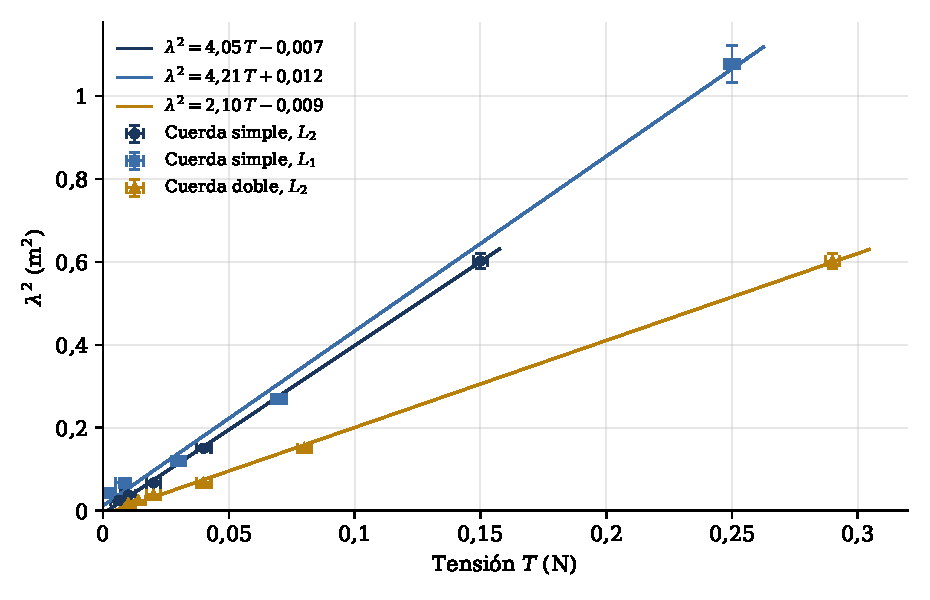
\includegraphics[width=0.82\textwidth]{ajustes_conjunto.pdf}
\caption{$\lambda^{2}$ frente a $T$ para los tres casos, con sus rectas de
ajuste. Barras de error: incertidumbres típicas $u(T)$ y $u(\lambda^{2})$.}
\end{figure}

\section*{Comentario}
Los tres ajustes son muy buenos ($r\geq\num{0,998}$) y las ordenadas son
compatibles con cero al \SI{95}{\percent}, como predice el modelo.
\begin{itemize}
  \item \emph{Distinta $L$, misma cuerda:} las pendientes de la cuerda simple en
    $L_2$ y $L_1$ (\num{4,05} y \num{4,21}) son compatibles, como se espera,
    porque la pendiente no depende de $L$.
  \item \emph{Misma $L$, distinta cuerda:} el cociente de pendientes en $L_2$ es
    $\num{4,05}/\num{2,10}=\num{1,93}$, muy próximo al valor 2 que corresponde a
    doblar la densidad.
  \item \emph{Densidad:} la cuerda simple da
    $\mu=\num{1,34 e-4}$ y $\num{1,28 e-4}\ \si{\kilogram\per\meter}$, y la doble,
    $\num{2,58 e-4}\ \si{\kilogram\per\meter}$, es decir,
    $\num{1,29 e-4}\ \si{\kilogram\per\meter}$ por hebra. Son algo mayores que
    el valor de la báscula, $\num{1,22 \pm 0,06 e-4}\ \si{\kilogram\per\meter}$,
    pero compatibles con él dentro de la incertidumbre, dominada por la escasa
    resolución de la pesada (\SI{0,01}{\gram} sobre \SI{0,06}{\gram}).
\end{itemize}
Los puntos de menor tensión (por debajo de \SI{0,01}{\newton}) son los menos
fiables, por estar cerca de la resolución del dinamómetro, pero su peso en la
pendiente es pequeño frente al de los modos $n=1$ y $n=2$.

\end{document}
